\textbf{Игровая интерпретация \psp:} на \psp можно смотреть с точки зрения теории игр. Из прошлого билета следует, что любая задача из \psp представляется в виде

\[ \exists y_1 \forall y_2 \ldots \exists/\forall y_{p(n)} V(x,y_1, \ldots, y_{p(n)}),\]

где $p(n)$ - некоторый полином от $n$ (число переменных может расти с ростом длины $x$). Данную формулу можно трактовать как игру с полиномиальным числом ходов: первый игрок делает ход $y_1$, второй - $y_2$ и т.д. $V(x, y_1, \ldots, y_{p(n)})$ указывает на то, кто победит в игре с начальной позицией $x$ и ходами $y_1, \ldots, y_{p(n)}$. Получаем

\[ \varphi \in \tqbf \Leftrightarrow \text{у первого игрока существует выигрышная стратегия}\]

Формализуем игру в города. Дан граф городов (предполагаем, что соединены как в игре: Архангельск-Кострома-Армавир-Ростов-Владивосток). Формально это значит, что если есть ребра $a \to c, b \to c, a \to d$, то есть и ребро $b \to d$. Два игрока двигают фишку вдоль ребер, при этом нельзя дважды переходить в одну и ту же вершину. Проигрывает тот, кто не может сделать ход. Стартовая вершина зафиксирована.

\begin{definition} 
    $\GG = \{(G, x)$ | из стартовой позиции $x$ на графе городов $G$ выиграет первый игрок\}. Название от \textit{Generalized Geography}.
\end{definition}

\begin{theorem}
    $\GG$ \psp-полон.
\end{theorem}

\begin{proof}
\begin{enumerate}
    \item Игра ациклична, так как нельзя создавать циклы, поэтому перед нами DAG. А на нем полным рекурсивным перебором можно перебрать все пути (они линейной от числа городов длины), то есть глубина рекурсии будет линейной, а на каждом состоянии нам важно помнить, а какие города мы уже посетили, что тоже полиномиально от длины входа. Значит принадлежность \psp доказана.
    
    \item Время полноты. Сведем $\tqbf$ к $\GG$. Будем сразу считать, что формула в 3-КНФ. Начнем строить граф, для этого для каждой переменной заведем четыре вершины $x^{in}, x^0, x^1, x^{out}$ и проведем между ними ребра $x^{in} \to x^0, x^{in}\to x^1, x^0\to x^{out}, x^1\to x^{out}$. 
    \begin{figure}[H]
        \centering
        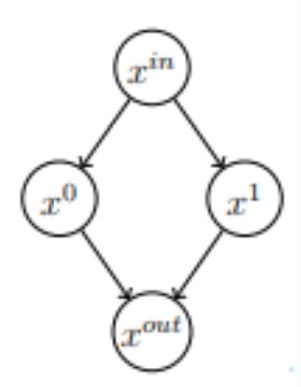
\includegraphics[width=0.2\textwidth]{images/gg.png}
    \end{figure}
    Теперь соединим эти <<ромбы>> в цепочку, проведя ребра $x_i^{out} \to x_{i + 1}^{in}$. Если $n$ (число переменных) нечетно, то сделаем еще одну вершину $y$ и сделаем ребро $x_n^{out} \to y$, а иначе $y = x_n^{out}$. Если $\varphi$ была конъюнкцией дизъюнктов $C_1, \ldots, C_m$, то заведем для каждого дизъюнкта по одной вершине и проведем $\forall j$ ребра $y \to C_j$. И, наконец, если дизъюнкт $C_j = (x_p^a \vee x_q^b \vee x_r^c)$, то проведем ребра $C_j \to x_p^a, C_j \to x_q^b, C_j \to x_r^c$ ($x_p^1 = x, x_p^0 = \overline{x}$). Начальной вершиной будет $x_1^{in}$.
    
    Покажем, что выполнимость формулы равносильна победе первого игрока. Будем считать, что ход $x_p^{in} \to x_p^{1 - a}$ равносилен тому, что теперь $x_p$ имеет значение $a$. Тогда первые $3n$ (или $3n-1$ для четного $n$) ходов первый и второй игроки выбирают значения всем переменным (за счет мостов $x_i^{out} \to x_{i + 1}^{in}$ между ромбами). 
    
    Если формула выполнима, то куда бы не пошел второй игрок из $y$ он проиграет, так как если формула выполнима, то в каждом дизъюнкте есть истинный литерал и первый игрок пойдет туда (так как на этапе построения набора мы специально ходили по инвертированным <<лживым>> вершинам). Из нее есть только путь в $x_j^{out}$, а они уже были пройдены, так что второму игроку некуда идти.
    
    Если формула невыполнима, то второй игрок может пойти из $y$ в ложный дизъюнкт, тогда первый игрок никуда сходить не сможет (так как все <<лживые>> вершины уже были пройдены) и он проиграет.
\end{enumerate}

\end{proof}

\begin{lemmanote}
    Даже в этой игре можно узреть аналогию на альтернирующие МТ и чередование состояний.
\end{lemmanote}